\section{Results}

	The testing and evaluation of our \textbf{informed} genetic algorithm took the form of three trials, each running for a series of 15 consecutive generations at 200 graphs per generation. Initial generations began with 20-nodes per graph, with 10\% of the node pool being dropped each generation to make room for new nodes. We also ran three trials without generational inheritance to simulate the process of simply randomly placing nodes on the graph. This \textbf{uninformed} system served as a baseline to compare our algorithm against. Each iteration of the uninformed tests involved generating a fresh population of graphs, each of which contained 10 nodes more than the previous, allowing for a predictable, linear growth in graph size. Additionally, it should be pointed out that our Unity Engine implementation color coded graph nodes based on inheritance. If a particular node was inherited from an ancestor, the node is colored red, otherwise if the node was freshly created during the previous crossover stage, the node is colored green. This color coding system allowed us to easily identify which attributes were inherited and which were freshly introduced.
	
	Although the informed trials did not quite reach 100\% A* satisfaction by the end of 15 generations, there are several advantages our genetic algorithm had over the uninformed method of simply placing nodes randomly in the maze. Primarily, as demonstrated in Figure 3, our informed genetic algorithm is consciousness of the graph size, avoiding over-saturation and preventing the node count from growing out of control. Graph size is critical to a well balanced A* waypoint graph. If a waypoint graph has far too many nodes, then A* will not be able to efficiently path find through the maze.
	
		\begin{figure}
			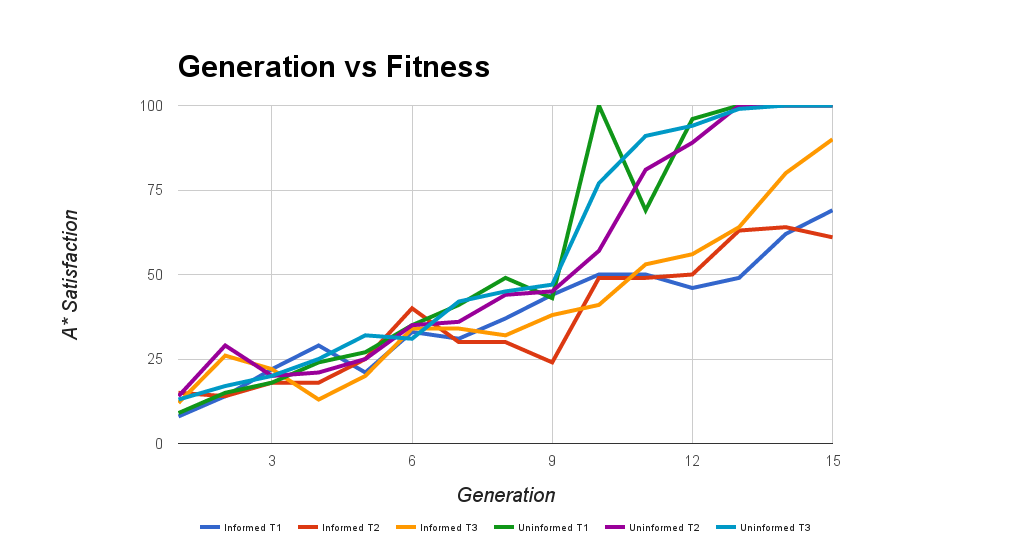
\includegraphics[width=1.2\columnwidth]{tests/genfitness}
			\caption{Red, Blue and Orange show the trials using our genetic algorithm, while Green, Purple and Cyan show trials using uninformed node placement.}
		\end{figure}
		
		\begin{figure}
			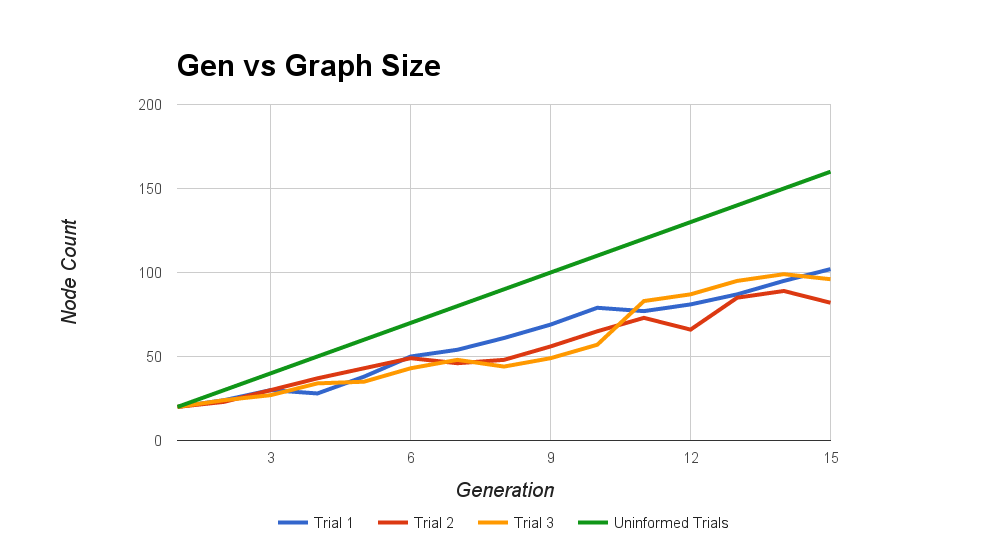
\includegraphics[width=1.2\columnwidth]{tests/gengraphsize}
			\caption{Green shows graph size growth for uninformed trials, while Red, Green and Orange show graph size for trials using our genetic algorithm. The uninformed system grows significantly faster than the genetic algorithm.}
		\end{figure}
		
		\begin{figure}
			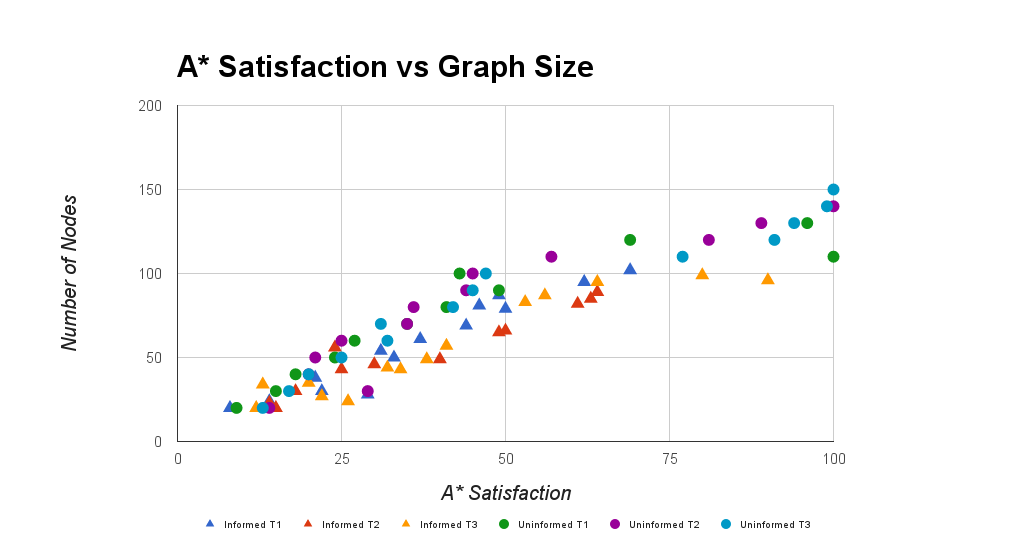
\includegraphics[width=1.2\columnwidth]{tests/satgraphsize}
			\caption{The Genetic algorithm (Triangles) consistently demonstrates that it requires far fewer nodes to achieve approximately the same A* Satisfaction rating as a completely uninformed system. (Circles)}
		\end{figure}
	
	Figure 3 demonstrates how the graph size scaled with each consecutive generation during each of the informed and uninformed trials. As the uninformed generations grew at a steady and predictable rate, the informed trials followed a more shallow linear progression, and in some cases decreased the number of nodes toward the end of the trial. Additionally, Figure 4 demonstrates how graph size changed with respect to A* satisfaction for each trial. We can see that in almost all cases, \textit{the genetic algorithm was able to build waypoint graphs that obtained the same A* satisfaction rating as the uninformed system, yet required far fewer nodes}. This was a huge achievement for the genetic algorithm system and really demonstrates one of it's ability to intelligently retain graph attributes that benefit it's fitness.
	